\documentclass{standalone}
\usepackage{tikz}
\usetikzlibrary{patterns, positioning}


\begin{document}
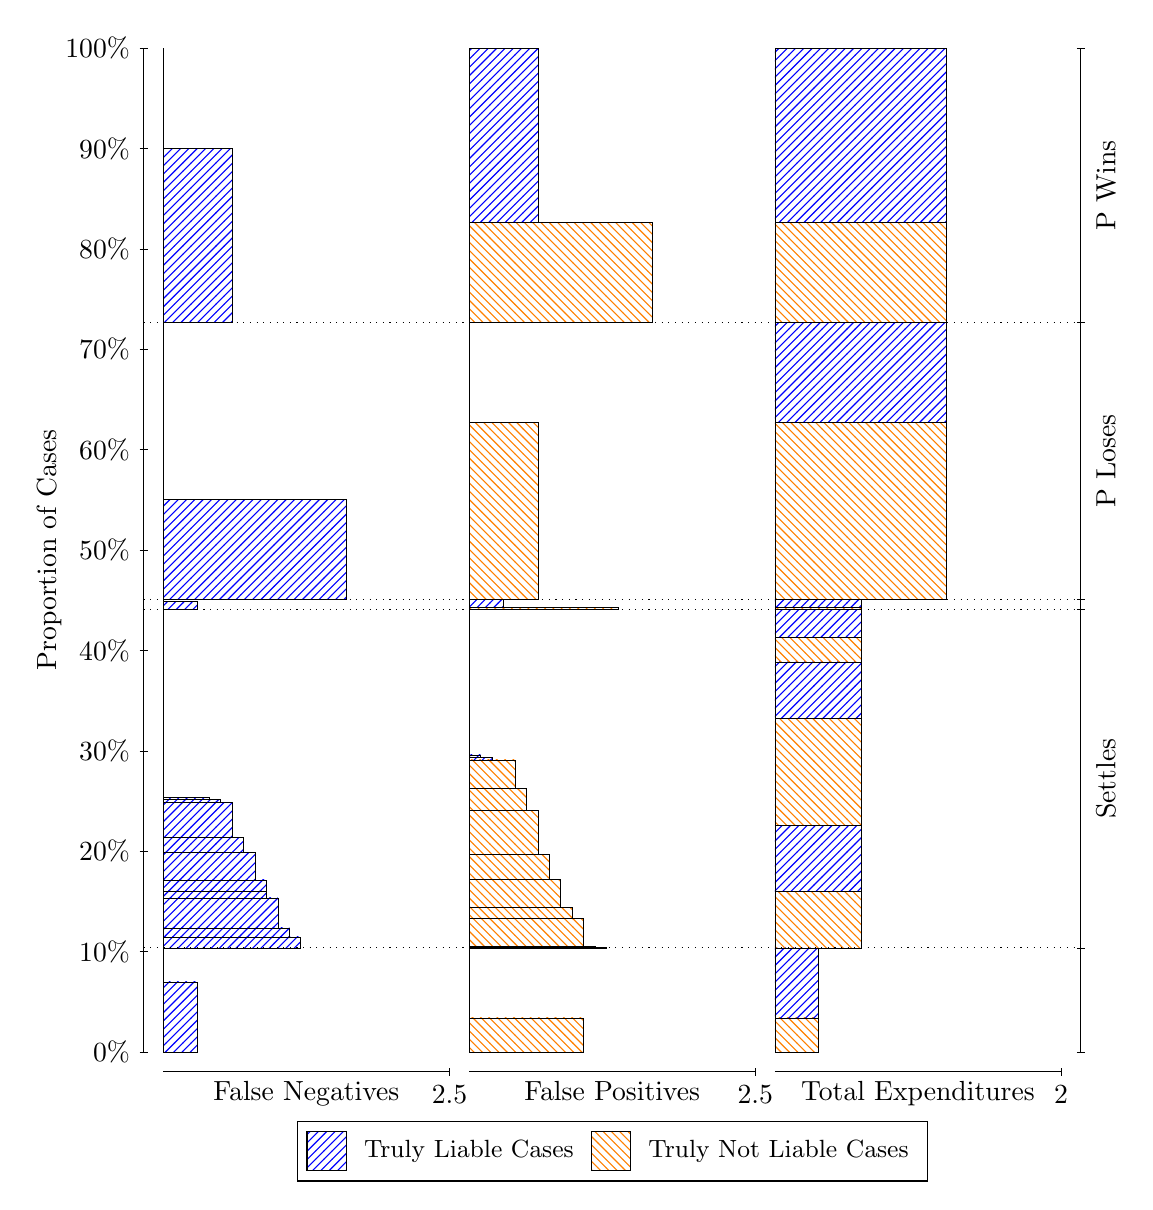
\begin{tikzpicture}
\draw[black, very thin] (1.5,1.75) -- (1.5,14.5);
\node[rotate=90, text=black, anchor=center] at (0.3, 8.125) {Proportion of Cases};
\draw[black, very thin] (1.45,1.75) -- (1.55,1.75);
\node[text=black, anchor=east] at (1.45, 1.75) {0\%};
\draw[black, very thin] (1.45,3.025) -- (1.55,3.025);
\node[text=black, anchor=east] at (1.45, 3.025) {10\%};
\draw[black, very thin] (1.45,4.3) -- (1.55,4.3);
\node[text=black, anchor=east] at (1.45, 4.3) {20\%};
\draw[black, very thin] (1.45,5.575) -- (1.55,5.575);
\node[text=black, anchor=east] at (1.45, 5.575) {30\%};
\draw[black, very thin] (1.45,6.85) -- (1.55,6.85);
\node[text=black, anchor=east] at (1.45, 6.85) {40\%};
\draw[black, very thin] (1.45,8.125) -- (1.55,8.125);
\node[text=black, anchor=east] at (1.45, 8.125) {50\%};
\draw[black, very thin] (1.45,9.4) -- (1.55,9.4);
\node[text=black, anchor=east] at (1.45, 9.4) {60\%};
\draw[black, very thin] (1.45,10.675) -- (1.55,10.675);
\node[text=black, anchor=east] at (1.45, 10.675) {70\%};
\draw[black, very thin] (1.45,11.95) -- (1.55,11.95);
\node[text=black, anchor=east] at (1.45, 11.95) {80\%};
\draw[black, very thin] (1.45,13.225) -- (1.55,13.225);
\node[text=black, anchor=east] at (1.45, 13.225) {90\%};
\draw[black, very thin] (1.45,14.5) -- (1.55,14.5);
\node[text=black, anchor=east] at (1.45, 14.5) {100\%};

\draw[black, very thin] (13.4,1.75) -- (13.4,14.5);
\draw[black, very thin] (13.35,1.75) -- (13.45,1.75);
\node[anchor=west] at (13.35, 1.75) {};
\draw[black, very thin] (13.35,3.0732) -- (13.45,3.0732);
\node[anchor=west] at (13.35, 3.0732) {};
\draw[black, very thin] (13.35,7.3681) -- (13.45,7.3681);
\node[anchor=west] at (13.35, 7.3681) {};
\draw[black, very thin] (13.35,7.5007) -- (13.45,7.5007);
\node[anchor=west] at (13.35, 7.5007) {};
\draw[black, very thin] (13.35,11.012) -- (13.45,11.012);
\node[anchor=west] at (13.35, 11.012) {};
\draw[black, very thin] (13.35,14.5) -- (13.45,14.5);
\node[anchor=west] at (13.35, 14.5) {};

\draw[black, very thin, pattern color=blue, pattern=north east lines] (1.75,1.75) rectangle (2.186,2.6401);
\draw[black, very thin, pattern color=orange, pattern=north west lines] (1.75,2.6401) rectangle (1.75,3.0732);
\draw[black, very thin, pattern color=blue, pattern=north east lines] (1.75,3.0732) rectangle (3.494,3.2104);
\draw[black, very thin, pattern color=blue, pattern=north east lines] (1.75,3.2104) rectangle (3.3487,3.3269);
\draw[black, very thin, pattern color=blue, pattern=north east lines] (1.75,3.3269) rectangle (3.2033,3.7078);
\draw[black, very thin, pattern color=blue, pattern=north east lines] (1.75,3.7078) rectangle (3.058,3.7949);
\draw[black, very thin, pattern color=blue, pattern=north east lines] (1.75,3.7949) rectangle (3.058,3.9344);
\draw[black, very thin, pattern color=blue, pattern=north east lines] (1.75,3.9344) rectangle (2.9127,4.2888);
\draw[black, very thin, pattern color=blue, pattern=north east lines] (1.75,4.2888) rectangle (2.7673,4.4741);
\draw[black, very thin, pattern color=blue, pattern=north east lines] (1.75,4.4741) rectangle (2.622,4.9173);
\draw[black, very thin, pattern color=blue, pattern=north east lines] (1.75,4.9173) rectangle (2.4767,4.9531);
\draw[black, very thin, pattern color=blue, pattern=north east lines] (1.75,4.9531) rectangle (2.3313,4.9815);
\draw[black, very thin, pattern color=orange, pattern=north west lines] (1.75,4.9815) rectangle (1.75,7.3681);
\draw[black, very thin, pattern color=blue, pattern=north east lines] (1.75,7.3681) rectangle (2.186,7.468);
\draw[black, very thin, pattern color=orange, pattern=north west lines] (1.75,7.468) rectangle (1.75,7.5007);
\draw[black, very thin, pattern color=blue, pattern=north east lines] (1.75,7.5007) rectangle (4.0753,8.7664);
\draw[black, very thin, pattern color=orange, pattern=north west lines] (1.75,8.7664) rectangle (1.75,11.012);
\draw[black, very thin, pattern color=blue, pattern=north east lines] (1.75,11.012) rectangle (2.622,13.223);
\draw[black, very thin, pattern color=orange, pattern=north west lines] (1.75,13.223) rectangle (1.75,14.5);
\draw[black, very thin, pattern color=orange, pattern=north west lines] (5.6333,1.75) rectangle (7.0867,2.1831);
\draw[black, very thin, pattern color=blue, pattern=north east lines] (5.6333,2.1831) rectangle (5.6333,3.0732);
\draw[black, very thin, pattern color=orange, pattern=north west lines] (5.6333,3.0732) rectangle (7.3773,3.0807);
\draw[black, very thin, pattern color=orange, pattern=north west lines] (5.6333,3.0807) rectangle (7.232,3.0936);
\draw[black, very thin, pattern color=orange, pattern=north west lines] (5.6333,3.0936) rectangle (7.0867,3.4501);
\draw[black, very thin, pattern color=orange, pattern=north west lines] (5.6333,3.4501) rectangle (6.9413,3.5911);
\draw[black, very thin, pattern color=orange, pattern=north west lines] (5.6333,3.5911) rectangle (6.796,3.9417);
\draw[black, very thin, pattern color=orange, pattern=north west lines] (5.6333,3.9417) rectangle (6.6507,4.2639);
\draw[black, very thin, pattern color=orange, pattern=north west lines] (5.6333,4.2639) rectangle (6.5053,4.8139);
\draw[black, very thin, pattern color=orange, pattern=north west lines] (5.6333,4.8139) rectangle (6.36,5.0958);
\draw[black, very thin, pattern color=orange, pattern=north west lines] (5.6333,5.0958) rectangle (6.2147,5.4598);
\draw[black, very thin, pattern color=blue, pattern=north east lines] (5.6333,5.4598) rectangle (5.924,5.4882);
\draw[black, very thin, pattern color=blue, pattern=north east lines] (5.6333,5.4882) rectangle (5.7787,5.5239);
\draw[black, very thin, pattern color=blue, pattern=north east lines] (5.6333,5.5239) rectangle (5.6333,7.3681);
\draw[black, very thin, pattern color=orange, pattern=north west lines] (5.6333,7.3681) rectangle (7.5227,7.4007);
\draw[black, very thin, pattern color=blue, pattern=north east lines] (5.6333,7.4007) rectangle (6.0693,7.5007);
\draw[black, very thin, pattern color=orange, pattern=north west lines] (5.6333,7.5007) rectangle (6.5053,9.7464);
\draw[black, very thin, pattern color=blue, pattern=north east lines] (5.6333,9.7464) rectangle (5.6333,11.012);
\draw[black, very thin, pattern color=orange, pattern=north west lines] (5.6333,11.012) rectangle (7.9587,12.289);
\draw[black, very thin, pattern color=blue, pattern=north east lines] (5.6333,12.289) rectangle (6.5053,14.5);
\draw[black, very thin, pattern color=orange, pattern=north west lines] (9.5167,1.75) rectangle (10.062,2.1831);
\draw[black, very thin, pattern color=blue, pattern=north east lines] (9.5167,2.1831) rectangle (10.062,3.0732);
\draw[black, very thin, pattern color=orange, pattern=north west lines] (9.5167,3.0732) rectangle (10.607,3.7931);
\draw[black, very thin, pattern color=blue, pattern=north east lines] (9.5167,3.7931) rectangle (10.607,4.6264);
\draw[black, very thin, pattern color=orange, pattern=north west lines] (9.5167,4.6264) rectangle (10.607,5.9837);
\draw[black, very thin, pattern color=blue, pattern=north east lines] (9.5167,5.9837) rectangle (10.607,6.7054);
\draw[black, very thin, pattern color=orange, pattern=north west lines] (9.5167,6.7054) rectangle (10.607,7.0148);
\draw[black, very thin, pattern color=blue, pattern=north east lines] (9.5167,7.0148) rectangle (10.607,7.3681);
\draw[black, very thin, pattern color=orange, pattern=north west lines] (9.5167,7.3681) rectangle (10.607,7.4007);
\draw[black, very thin, pattern color=blue, pattern=north east lines] (9.5167,7.4007) rectangle (10.607,7.5007);
\draw[black, very thin, pattern color=orange, pattern=north west lines] (9.5167,7.5007) rectangle (11.697,9.7464);
\draw[black, very thin, pattern color=blue, pattern=north east lines] (9.5167,9.7464) rectangle (11.697,11.012);
\draw[black, very thin, pattern color=orange, pattern=north west lines] (9.5167,11.012) rectangle (11.697,12.289);
\draw[black, very thin, pattern color=blue, pattern=north east lines] (9.5167,12.289) rectangle (11.697,14.5);
\draw[black, dotted] (1.5,3.0732) -- (13.4,3.0732);
\draw[black, dotted] (1.5,7.3681) -- (13.4,7.3681);
\draw[black, dotted] (1.5,7.5007) -- (13.4,7.5007);
\draw[black, dotted] (1.5,11.012) -- (13.4,11.012);
\draw[black, very thin] (1.75,1.5) -- (5.3833,1.5);
\node[text=black, anchor=north] at (3.5667, 1.5) {False Negatives};
\draw[black, very thin] (5.3833,1.45) -- (5.3833,1.55);
\node[text=black, anchor=north] at (5.3833, 1.45) {2.5};

\draw[black, very thin] (5.6333,1.5) -- (9.2667,1.5);
\node[text=black, anchor=north] at (7.45, 1.5) {False Positives};
\draw[black, very thin] (9.2667,1.45) -- (9.2667,1.55);
\node[text=black, anchor=north] at (9.2667, 1.45) {2.5};

\draw[black, very thin] (9.5167,1.5) -- (13.15,1.5);
\node[text=black, anchor=north] at (11.333, 1.5) {Total Expenditures};
\draw[black, very thin] (13.15,1.45) -- (13.15,1.55);
\node[text=black, anchor=north] at (13.15, 1.45) {2};


\node[text=black, centered, rotate=90] at (13.72, 5.2206) {Settles};

\node[text=black, centered, rotate=90] at (13.72, 9.2564) {P Loses};
\node[text=black, centered, rotate=90] at (13.72, 12.756) {P Wins};

\draw (7.449999999999999,1.5) node[draw=none] (baseCoordinate) {};
\begin{scope}[align=center]
        \matrix[scale=0.5, draw=black, below=0.5cm of baseCoordinate, nodes={draw}, column sep=0.1cm]{
            \node[rectangle, draw, minimum width=0.5cm, minimum height=0.5cm, pattern color=blue, pattern=north east lines] {}; &
            \node[draw=none, font=\small, text=black] (B) {Truly Liable Cases}; &
            \node[rectangle, draw, minimum width=0.5cm, minimum height=0.5cm, pattern color=orange, pattern=north west lines] {}; &
            \node[draw=none, font=\small, text=black] (B) {Truly Not Liable Cases}; \\
            };
\end{scope}

\end{tikzpicture}
\end{document}